\icode{E-MD-CA-L2-261111-002}
如图所示，一质量 \(M =\) \,\qty{40}{kg}、长 \(L =\) \,\qty{2.5}{m}的平板车静止在光滑的水平地面上。一质量 \(m =\) \,\qty{10}{kg}可视为质点的滑块，以 \(v_0 =\) \,\qty{5}{m/s}的初速度从左端滑上平板车，滑块与平板车间的动摩擦因数 \(\mu = 0.4\)，取 \(g =\) \,\qty{10}{m/s^2}。	
\begin{enumerate}
	\item 分别求出滑块在平板车上滑行时，滑块与平板车的加速度大小；
	\item 计算说明滑块能否从平板车的右端滑出。
\end{enumerate}

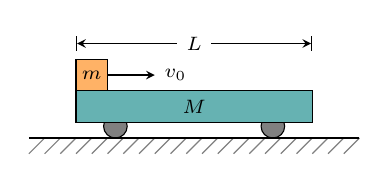
\begin{tikzpicture}[>=stealth,font=\scriptsize]
	\draw[fill=orange!60] (0,.4) rectangle(.4,.8)node[midway]{\(m\)};
    \draw[fill=gray] (.5,-.05) circle(.15) (2.5,-.05) circle(.15);
	\draw[fill=teal!60] (0,0) rectangle(3,.4)node[midway]{\(M\)};
	\draw[->] (.4,.6)--++(.6,0)node[right]{\(v_0\)};
	\draw[|<->|] (0,1)--node[fill=white]{\(L\)}(3,1);
	\foreach \x in {-.6,-.4,...,3.6}
		\draw[gray] (\x,-.4)--++(.2,.2);
	\draw[thick] (-.6,-.2)--(3.6,-.2);
\end{tikzpicture}
\begin{answer}
	（1）\(a_1 =\) \,\qty{4}{m/s^2}\: \(a_2 =\) \,\qty{1}{m/s^2}（2）恰好滑下
\end{answer}